\documentclass{article}
\usepackage{v-test-paper}
\title{\textsc{Kinematics}}
\date{February 22, 2024}

\newcommand{\itemstared}{\refstepcounter{enumi}\item[$^\star$\theenumi.]}
\usetikzlibrary{matrix,  positioning, patterns, backgrounds}
\renewcommand{\ans}{\quad}


\tikzstyle{root} = [rectangle, rounded corners, 
minimum width=3cm, 
minimum height=0.7cm,
text centered, 
draw, 
font=\scshape,
]
\tikzstyle{child} = [rectangle, rounded corners, 
inner sep=2mm,
text centered, 
draw, 
font=\itshape,
text width=3.25cm,
]

\tikzstyle{child-branch} = [
    rectangle, 
    rounded corners, 
    inner sep=2mm,
    text centered, 
    draw, 
    font=\itshape,
    text width=2.5cm,
    level distance=5mm,
]



\tikzstyle{arrow} = [thick,->,>=latex]


\begin{document}
\maketitle
\begin{center}
\begin{tikzpicture}[node distance=2cm]

\matrix [column sep=5mm,row sep=10mm]
{
&\node (root) [root] {Kinematics};\\
\node (child-left)[child] {Position}; &
\node (child-center)[child] {Graphs}; &
\node (child-right)[child]{Relative Motion};\\
\node (child-left-b)[child] {Velocity}; & &\\
\node (child-left-bb)[child] {Acceleration}; &
\node (child-center-b)[child]{Position-time Velocity-time Acceleration-time Velocity-position}; &
\node[child-branch](child-right-bl)at ($(child-right.south)+(-1.5, 0)$){Uniform Velocity};
\node[child-branch](child-right-br)at ($(child-right.south)+(1.5, 0)$){Non-Uniform Velocity};\\
\node[child-branch](child-left-bbl)at ($(child-left-bb.south)+(-1.5, 0)$){Non-Uniform Accelleration};
\node[child-branch](child-left-bbr)at ($(child-left-bb.south)+(1.5, 0)$){Uniform Acceleration}; & &
\node[child-branch](child-right-bbl)at ($(child-right-bl.south)+(0, 0)$){Rain-man River-boat Wind-aeroplane};\\
};

\draw [arrow] (root) -| (child-left);
\draw [arrow] (root) -| (child-right);
\draw [arrow] (child-left) --(child-left-b);
\draw [arrow] (root)--(child-center);
\draw [arrow] (child-center) -- (child-center-b);
\draw [arrow] (child-right) -- (child-right-bl);
\draw [arrow] (child-right) -- (child-right-br);
\draw [arrow] (child-left-bb)--(child-left-bbl);
\draw [arrow] (child-left-bb)--(child-left-bbr);
\draw [arrow] (child-left-b)--(child-left-bb);
\draw [arrow] (child-right-bl)--(child-right-bbl);
\end{tikzpicture}
\end{center}

\begin{center}
    \textsc{Problems}
\end{center}
\begin{enumerate}
    \item The acceleration time graph of a particle moving in a straight line is as shown in the figure. The velocity of the particle at time $t=0$ is 2 m/s. The velocity after 2 seconds will be
    \begin{center}
        \begin{tikzpicture}
            \draw [->, thick](-1, 0)--(5, 0) node[below]{t($s$)};
            \draw [->, thick](0, -1)--(0, 3) node[left]{a($m/s^2$)};
            \draw (0, 0)--(2, 2)--(4, 0) node[below]{2};
            \draw[dashed] (0, 2)node[left]{4}--(2, 2)--(2, 0) node[below]{1};
        \end{tikzpicture}
    \end{center}
    \begin{tasks}(4)
        \task $6 \mps$\ans
        \task $4 \mps$
        \task $2 \mps$
        \task $8 \mps$
    \end{tasks}

    \itemstared The displacement $x$ of a particle moving along a straight line, at time $t$ is given by $x = \dfrac{a}{b}(1-e^{-bt})$ where $a$ and $b$ are real positive constants. Therefore :
    \begin{tasks}(1)
        \task the graph of velocity vs displacement is a straight line with negatice slope \ans
        \task the velocity and acceleration of the particle at $t=0$ are $a$ and $(-ab)$ respectively \ans
        \task the particle cannot reach a point at a distance $x'$ from its starting point if $x' >a/b$ \ans
        \task the particle will return to its starting point $ t \to \infty$
    \end{tasks}
 
    
    
    \item The velocity versus time graph for a particle moving along a straight line is shown below. Select the correct option(s).
        \begin{center}
        \begin{tikzpicture}
        \draw [-Stealth](0, -2)--(0, 2) node[left]{v(m/s)};
        \draw [-Stealth](-0.5, 0)--(6, 0) node[right]{t(s)};
        \draw (1, -1.5)--(5,1.5);
        \draw[thick,dashed](1,0)--(1,-1.5);
        \draw[thick,dashed](5,0)--(5,1.5);
        \node at (1,0)[below left]{$1$};
        \foreach \x in {3,5,...,5}
                     \draw (\x,0) -- (\x,0)
                    node[anchor=north] {\x};
        \end{tikzpicture}
        \end{center}
        \begin{tasks}(2)
            \task speed of particle is same at $2 \s$ and $4 \s$\ans
            \task velocity of particle at $t=2 \s$ will be $1 \mps$
            \task $\int_{t=1}^{t=5}v\d{t}$ is zero \ans
            \task velocity of particle is zero at $t=2 \s$ 
        \end{tasks}

    \itemstared A particle is moving in x-y plane. At certain instant of time, the components of its velocity and acceleration are as follows. $v_x=3 \mps$, $v_y=4 \mps$, $a_x=2 \mpss$ and $a_y=1 \mpss$. The rate of change of speed at this moment is:
        \begin{tasks}(2)
        \task $\sqrt{10} \mpss$
        \task $4 \mpss$
        \task $10 \mpss$
        \task $2 \mpss$\ans
        \end{tasks}

    \item A particle is moving in a straight line with initial velocity $u$ and uniform acceleration $f$. If the sum of the distances travelled in $t^{\textit{th}}$ and $(t+1)^{\text{th}}$ seconds is 100 cm, then its velocity after $t$ seconds, in cm/s, is :
        \begin{tasks}(4)
            \task $20$
            \task $30$
            \task $50$\ans
            \task $80$
        \end{tasks}

        \item A bead is free to slide down a smooth straight frictionless rod between point $A$ and $B$ on a vertical circle of radius $R$. If the bead starts from rest at $A$, the highest point on the circle, the time to arrive at $B$ is : 
        \begin{multicols}{2}
        \begin{tasks}(1)
            \task $2\sqrt{\dfrac{R}{g}}$\ans
            \task $\sqrt{\dfrac{2R}{g}\tan \theta}$
            \task $2\sqrt{\dfrac{R}{g}\tan \theta}$
            \task None of these
        \end{tasks}
        \begin{center}
            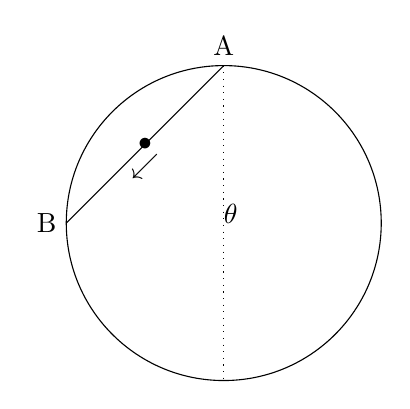
\begin{tikzpicture}
                \draw (0, 0) circle[radius=2];
                \draw[dotted] (0, 2)coordinate (a) node[above]{A}--(0,-2)coordinate (c);
                \draw (0, 2)--(-2,0)coordinate (b) node[left]{B} node[midway]{$\bullet$} node[midway, below]{$\swarrow$};
                \tzanglemark(b)(a)(c){$\theta$}
            \end{tikzpicture}
        \end{center}
        \end{multicols}

    \item A particle is moving along $X-$axis whose position is given by $x=4+9t + \dfrac{t^3}{3}$. Mark the correct statement(s) in relation to its motion :
        \begin{tasks}(1)
            \task Direction of motion is not changing at any of the instants\ans
            \task Direction of motion is changing at $t=3\s$
            \task for $0 < t < 3 \s$, the particle is slowing down
            \task for $0 < t <3 \s$, the particle is speeding up\ans
        \end{tasks}

    \item The motion of a body falling from rest in a resisting medium is described by the equation $\dfrac{\d{v}}{\d{t}} = a -bv$ where $a$ and $b$ are constants. The velocity at any time $t$ is :
        \begin{tasks}(2)
            \task $v_t=\dfrac{a}{b}\left(1-e^{-bt}\right)$\ans
            \task $v_t=\dfrac{b}{a}e^{-bt}$
            \task $v_t=\dfrac{a}{b}\left(1+e^{-bt}\right)$
            \task $v_t=\dfrac{b}{a}e^{bt}$
        \end{tasks}
        
    \item A particle moves in the x-y plane with a velocity $v_x=8t-2$ and $v_y=2$. If it passes through the point $x=14$ and $y=4$ at $t=2\s$, the equation of its trajectory is :
        \begin{tasks}(2)
            \task $x=y^2-y+2$\ans
            \task $x=y^2-2$
            \task $x=y^2+y-6$
            \task None of these
        \end{tasks}
 
    \item Two particles $1$ and $2$ are thrown in the directions shown in figure simultaneously with velocities $5\mps$ and $20\mps$. Initially, particle $1$ is at height $20\m$ from the ground. Taking upwards as the positive direction, find the time when the particles will collide.
        \begin{center}
            \begin{tikzpicture}
                \pic (0, 0)(ground) {frame=2cm};
                \begin{scope}[yshift=5pt]
                    \tzdot*(0, 0)(10pt)
                    \tzline+[->](ground-center)(0, 1){$20\mps$}[r]
                    \tzdot*<0, 3>(0, 0)(10pt)
                    \tzline+[->]<0, 3>(0, 0)(0, -1){$5\mps$}[r]
                \end{scope}
                \tzline[|-|](-1, 0)(-1, 3.2){$20\m$}[midway, l]
            \end{tikzpicture}
        \end{center}
        \begin{tasks}(2)
            \task $\dfrac{20}{25}\s$\ans
            \task $\dfrac{20}{15}\s$
            \task $\dfrac{20}{20}\s$
            \task none of these
        \end{tasks}
        
    \item A ball is thrown upwards from the top of a tower $40\m$ high with a velocity of $10\mps$. Find the time when it strikes the ground.
        Take $g=10\mpss$.
        \begin{center}
            \begin{tikzpicture}[test-paper]
                \pic (0, 0)(G){frame=2cm};
                \tzpath[pattern=bricks, draw]
                    (-0.5, 0)(0.5, 0)(0.5, 2)(-0.5, 2)(-0.5, 0);
                \tzline[|-|](-1, 0)(-1, 2){$40\m$}[midway, l]
                \begin{scope}[yshift=6pt]
                \tzdot*(0.5, 2)(10pt) 
                \tzline+[->](0.5, 2)(0, 1){$10\mps$}[r]
                \end{scope}
                
            \end{tikzpicture}
        \end{center}
        \begin{tasks}(2)
            \task $2\s$
            \task $4\s$\ans
            \task $3\s$
            \task none of these
        \end{tasks}

        \item Which of the following graphs correctly represents velocity-time relationship for a particle released from rest to fall freely under gravity ?
        \def\OptionA{
            \begin{tikzpicture}
                \tzaxes(0, 0)(2, 2){$t$}{$v$}
                \tzline(0, 0)(1.5, 1.5)
            \end{tikzpicture}
        }

        \def\OptionB{
            \begin{tikzpicture}
                \tzaxes(0, 0)(2, 2){$t$}{$v$}
                \tzline(0, 1.5)(1.5, -0.5)
            \end{tikzpicture}
        }

        \def\OptionC{
            \begin{tikzpicture}
                \tzaxes(0, 0)(2, 2){$t$}{$v$}
                \tzlines(0, 0)(0.8, 1)(1.6, 0);
            \end{tikzpicture}
        }

        \def\OptionD{
            \begin{tikzpicture}
                \tzaxes(0, 0)(2, 2){$t$}{$v$}
                \tzlines(0, 1)(0.8, 0)(1.6, 1);
            \end{tikzpicture}
        }

        \begin{tasks}(2)
            \task \OptionA\ans
            \task \OptionB
            \task \OptionC
            \task \OptionD
        \end{tasks}
        

        \item Which of the following is the correct option for the given $s-t$ graph ?
        \begin{center}
            \begin{tikzpicture}
                \tzaxes(0, 0)(6, 4.5){$t$}{$s$}
                \tztos"curve"(0, 0)[out=0, in=270]
                            (1.5, 1.5)[out=90, in=180]
                            (3, 3)[out=0, in=180]
                            (4.5, 4);
                \tzvXpointat*{curve}{1.5}{$A$}[0](3pt)
                \tzvXpointat*{curve}{2.25}{$B$}[-90](3pt)
                \tzvXpointat*{curve}{3.35}{$C$}[-90](3pt)
            \end{tikzpicture}   
        \end{center}
        \begin{tasks}(2)
            \task velocity at $A$ is +ve but acceleration is -ve
            \task velocity at $B$ is +ve but acceleration is -ve\ans
            \task velocity at $C$ is +ve but acceleration is -ve
            \task none of these
        \end{tasks}

        \item A boatman wants to cross a river of width $w$ along the shortest path. If $|\Vec{v}_b|=5$ and $|\Vec{v}_r|=4$, then how much time it'll take to cross this river ?
        \begin{center}
        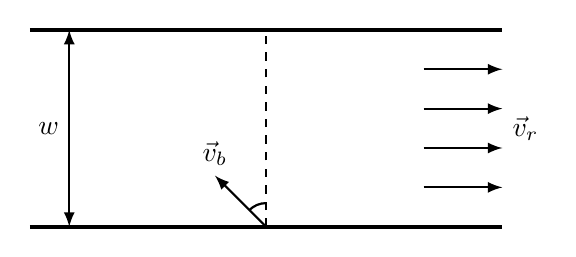
\begin{tikzpicture}[>=latex, thick]
        %\draw[->] (0, 0)--((5, 0);
        %\fill[pattern=north east lines](0, 0) rectangle (4, -0.5);
        \draw[ultra thick] (-3, 0)--(3, 0) (-3, 2.5)--(3, 2.5);
        \foreach \y in {0.5, 1.0,..., 2}{
        \draw[->] (2, \y)--(3, \y);
        };
        \node at (3, 1.25)[right]{$\vec{v}_r$};
        \draw[dashed](0,0)--(0, 2.5);
        \draw[->](0, 0)--(-0.65, 0.65) node[left, above]{$\vec{v}_b$};
        \draw (0, 0.3) arc (90:135:0.3);
        \draw[<->](-2.5, 0)--(-2.5, 2.5) node[left, midway]{$w$};
        \end{tikzpicture}
        \end{center}
        \begin{tasks}(2)
            \task $\dfrac{w}{3}$\ans
            \task $\dfrac{w}{4}$
            \task $4w$
            \task $3w$
        \end{tasks}

        \item A girl is walking on a horizontal road with a speed of $3\mps$. Raindrops are falling vertically downward with speed of $4\mps$ w.r.t. ground. In which direction the girl should hold her umbrella to keep the rain away ?
\begin{tasks}(2)
    \task $\dfrac{3}{5}\hat{i}+\dfrac{4}{5}\hat{j}$\ans
    \task $\dfrac{5}{3}\hat{i}+\dfrac{5}{4}\hat{j}$
    \task $\dfrac{4}{5}\hat{i}+\dfrac{3}{5}\hat{j}$
    \task none of these
\end{tasks}

\item Position of a particle varies as 
\[x=\dfrac{t^3}{3}-t^2+t\]
Which of the following $v-t$ graph is correct for the above equation ?
\def\OptionA{
    \begin{tikzpicture}
        \tzaxes(0, 0)(2.5, 2){$t(s)$}{$v(\mps)$}
        \tztos(0, 1)[out=300, in=180]
                (1, 0)[out=0, in=240]
                (2, 1);
    \end{tikzpicture}
}
\def\OptionB{
    \begin{tikzpicture}
        \tzaxes(0, 0)(2.5, 2){$t(s)$}{$v(\mps)$}
        \tztos(0, 0)[out=60, in=180]
                (1, 1)[out=0, in=120]
                (2, 0);
    \end{tikzpicture}
}
\def\OptionC{
    \begin{tikzpicture}
        \tzaxes(0, 0)(2.5, 2){$t(s)$}{$v(\mps)$}
        \tztos<0, 0.5>(0, 1)[out=300, in=180]
                (1, 0)[out=0, in=240]
                (2, 1);
    \end{tikzpicture}
}
\def\OptionD{
    \begin{tikzpicture}
        \tzaxes(0, 0)(2.5, 2){$t(s)$}{$v(\mps)$}
        \tztos<0, 0.5>(0, 0)[out=60, in=180]
                (1, 1)[out=0, in=120]
                (2, 0);
    \end{tikzpicture}
}
    \begin{tasks}(2)
        \task \OptionA\ans
        \task \OptionB
        \task \OptionC
        \task \OptionD
    \end{tasks}

\item The motion of a particle along a straight line is described by equation
\[x=8+12t-t^3\]
where, $x$ is in metre and $t$ in second. The retardation of the particle when its velocity becomes zero, is
\begin{tasks}(2)
    \task $24\mpss$
    \task zero
    \task $6\mpss$
    \task $12\mpss$\ans
\end{tasks}

\item A rod AB is shown in the figure. End $A$ of the rod is fixed on the ground and can rotate about it. Block is moving with velocity $2\mps$ towards right. The velocity of the end $B$ of the rod at the instant shown in the figure is :
    \begin{center}
        \begin{tikzpicture}
            \tzcoor*(-2, 0)(A){$A$}[a]
            \tzcoor(1, 2)(B){$B$}[a]
            \pic at (0, 0)(ground){frame=6cm};
            \tzrectangle[pattern=north east lines](1, 0)(1.5, 2);
            \tzline+[->](1.5, 1.75)(1, 0){$2\mps$}[r]
            \tzline[line width=0.5mm, cap=round](A)(B);
            \tzanglemark(0, 0)(A)(B){$30^\circ$}(18pt)
        \end{tikzpicture}
    \end{center}
    \begin{tasks}(2)
        \task $2\sqrt{3}\mps$
        \task $\sqrt{3}\mps$
        \task $3\sqrt{3}\mps$
        \task $4\mps$\ans
    \end{tasks}

    \begin{center}
        \textsc{Paragraph Type}
    \end{center}
    A situation is shown in which two objects A and B start their motion from same point in same direction. The graph of their velocities against time is drawn. $u_A$ and $u_B$ are the initial velocities of A and B respectively. $T$ is the time at which their velocities become equal after start of motion. You cannot use the data of one question while solving another question of the same set. So all the questions are independent of each other.
    \begin{center}
        \begin{tikzpicture}
            \tzaxes(-0.5, -0.5)(5, 3.5){$t$}{$v$}
            \tzcoor(0, 1)(A){$u_A$}[l]
            \tzcoor(0, 3)(B){$u_B$}[l]
            \tzline"VA"(A)(4, 3){$A$}[a]
            \tzline"VB"(B)(4, 0.5){$B$}[b]
            \tzXpoint*{VA}{VB}(X)
            \tzprojx(X){$T$}
        \end{tikzpicture}
    \end{center}
    \item If the value of $T$ is $4\s$, then the time after which $A$ will overtake $B$ is :
    \begin{tasks}(2)
        \task $8\s$\ans
        \task $12\s$
        \task $16\s$
        \task data insufficient
    \end{tasks}

    \item Let $v_A$ and $v_B$ be the velocities of $A$ and $B$ respectively at the moment $A$ and $B$ meet after start of motion.  If $u_A=5\mps$ and $u_B=15\mps$, then the magnitude of the difference of velocities of $A$ and $B$ is
    \begin{tasks}(2)
        \task $10\mps$\ans
        \task $5\mps$
        \task $15\mps$
        \task $20\mps$
    \end{tasks}

    \item After $10\s$ of the start of motion of both the objects, find the velocity of $A$ if $u_A=6\mps$, $u_B=12\mps$ and at $T$ the velocity of $A$ is $8\mps$ and $T=4\s$
    \begin{tasks}(2)
        \task $10\mps$
        \task $12\mps$
        \task $15\mps$
        \task None of these \ans
    \end{tasks}

    



\end{enumerate}


\pagebreak

\begin{center}
\texttt{Answer Key}
\begin{multicols}{5}
\begin{enumerate}
\item (b)
\item (b)
\item (a)
\item (b)
\item (d)
\item (b)
\item (c)
\item (a), (b)
\item (c)
\item (a), (b), (c), (d)
\end{enumerate}
\end{multicols}
\end{center}






\end{document}